\documentclass[conference]{IEEEtran}
\usepackage{graphicx}
\usepackage{booktabs}
\usepackage{amsmath,amssymb}
\usepackage{array}
\usepackage{url}
\usepackage[hidelinks]{hyperref}
\begin{document}
\title{Do Explicit Cross-Sensor Consistency Features Help? A Leakage-Controlled Benchmark for Coordinated Multi-Channel False Data Injection Detection in IoMT}
\author{
\IEEEauthorblockN{Prabakar P, 22MIS0527}
\IEEEauthorblockA{Department of Software and Systems Engineering, School of Computer Science Engineering and Information Systems\\Vellore Institute of Technology, Vellore, India}
}
\maketitle
\begin{abstract}
Coordinated multi-channel false data injection (FDI) attacks manipulate several physiological sensors simultaneously so that each channel remains individually plausible while the joint relationship between channels is violated. A natural hypothesis is that explicitly modelling cross-sensor consistency improves detection over naive multi-channel fusion. We test this hypothesis under a leakage-controlled protocol on two public datasets, the PhysioNet/CinC 2012 ICU corpus and the WESAD wearable corpus: subject- and record-level splits (70/15/15), train-only normalisation, thresholds calibrated on validation data, three random seeds, and hierarchical paired bootstrap with McNemar testing. We compare three architectures that share an identical temporal encoder: (A) naive flat fusion, (B) graph-only message passing over a physiology-informed channel graph, and (C) cross-sensor consistency modelling (CSCM), which augments the relation input with explicit pairwise difference and element-wise product features. On the clinical corpus, graph-only message passing is the strongest model (F1 0.8863$\pm$0.0031, AUPRC 0.9583, AUROC 0.9029) and is significantly better than naive fusion at one seed, whereas the explicit consistency features of CSCM do not produce a consistent benefit and are significantly worse than graph-only at another seed. On the wearable corpus the three models are statistically indistinguishable and AUROC is near chance. We conclude that graph structure, not hand-engineered consistency arithmetic, is the useful inductive bias, and we report this largely null result as a reproducible benchmark.
\end{abstract}
\begin{IEEEkeywords}
Internet of Medical Things; false data injection; cross-sensor consistency; graph neural networks; physiological time series; anomaly detection; reproducibility; negative results
\end{IEEEkeywords}
\section{Introduction}
The Internet of Medical Things (IoMT) places networked sensors at the bedside and on the body, continuously streaming physiological signals into clinical and wearable monitoring systems. Because these signals increasingly drive automated alerts and decision support, their integrity is a safety property rather than a convenience. A false data injection (FDI) attack that corrupts a physiological reading can therefore cause a missed deterioration or a spurious alarm. The security and privacy surface of the IoMT has been extensively surveyed \cite{alsubaei2017}, and FDI attacks were first formalised in the cyber-physical power-grid setting \cite{liu2011}, \cite{mo2012}.
Most deployed monitors evaluate each channel independently and raise an alarm when a value crosses a physiological bound. This is precisely the assumption that a coordinated adversary defeats. In a coordinated multi-channel attack the adversary injects correlated perturbations into several sensors at once, choosing magnitudes small enough that every individual channel remains biologically plausible. The marginal distributions survive; the joint, cross-sensor relationship does not.
It is therefore natural to hypothesise that a detector which explicitly models cross-sensor consistency will outperform one that merely concatenates channels. This paper tests that hypothesis rather than assuming it. We build three architectures on an identical temporal encoder and compare them under strict controls: subject- and record-level data splitting, train-only normalisation, validation-calibrated decision thresholds, three random seeds, and hierarchical paired bootstrap confidence intervals with McNemar testing \cite{efron1993}, \cite{dietterich1998}.
Our central finding is negative and, we argue, useful. Physiological graph structure is a genuine inductive bias: on the clinical dataset it improves detection, and the improvement is statistically visible at one seed. Adding hand-engineered consistency arithmetic on top of that graph --- absolute pairwise differences and element-wise products --- does not help consistently, and at one seed it significantly hurts. On the wearable dataset, where the signals are already clean and synchronised, none of the three models separates from the others and discrimination is close to chance.
The contributions of this work are:
\begin{itemize}
\item A leakage-controlled benchmark for coordinated multi-channel FDI detection on two public datasets drawn from different physiological contexts (clinical ICU and wearable laboratory monitoring).
\item A controlled three-way ablation (naive fusion vs. graph-only message passing vs. explicit cross-sensor consistency features) in which the temporal encoder is frozen across all three models.
\item A statistical analysis that reports effect sizes with subject-level bootstrap confidence intervals and paired McNemar tests, showing where differences are reliable and where they are not.
\item A failure analysis that identifies the boundary conditions of graph-based detection: sparse positive channels, physiological missingness, and coordinated attacks that remain harder than single-channel ones.
\item A reproducible, openly specified protocol so that the largely null result can be confirmed or refuted rather than asserted.
\end{itemize}
\section{Related Work}
\subsection{False Data Injection in Cyber-Physical Systems}
FDI attacks were introduced for state estimation in power grids, where an adversary who knows the system topology can inject a consistent bias that is invisible to residual-based bad-data detection \cite{liu2011}. The broader security properties of such cyber-physical infrastructures are surveyed by Mo et al. \cite{mo2012}. The IoMT inherits the same threat model with a different physical substrate: the adversary attacks the integrity of measurements that a human or a downstream model will trust.
\subsection{Anomaly Detection for Physiological Time Series}
Deep anomaly detection for time series is a large field, surveyed by Chalapathy and Chawla \cite{chalapathy2019}. Recurrent architectures, in particular the gated recurrent unit \cite{cho2014} and the LSTM \cite{hochreiter1997}, remain standard temporal encoders, and convolutional feature extractors are commonly stacked in front of them. Our shared encoder follows this pattern; the object of study is not the encoder but the fusion mechanism that sits above it.
\subsection{Graph and Relational Models}
Graph neural networks provide a structural inductive bias by computing messages between related entities \cite{kipf2017}, \cite{gilmer2017}, and the general argument for relational inductive biases is made by Battaglia et al. \cite{battaglia2018}. Our graph-only model is a minimal message-passing network over a physiology-informed channel graph, implemented with PyTorch \cite{paszke2019} and PyTorch Geometric \cite{fey2019} primitives.
\subsection{Datasets and Positioning}
We use two public datasets that represent opposite ends of IoMT monitoring: the PhysioNet/Computing in Cardiology Challenge 2012 ICU corpus \cite{silva2012} and the WESAD wearable corpus \cite{schmidt2018}. To our knowledge the specific question posed here --- whether explicit, hand-engineered cross-sensor consistency features improve on graph message passing for coordinated FDI detection --- has not been answered under a leakage-controlled protocol. Our contribution is therefore a benchmark and a carefully bounded negative result, not a claim of state-of-the-art accuracy.
\section{Problem Formulation and Threat Model}
Consider an IoMT deployment monitoring a patient through C heterogeneous sensors. At time step t the system observes a vector x\_t $\in$ $\mathbb{R}$^C, and over a window of length T it processes the matrix X $\in$ $\mathbb{R}$^(T$\times$C). Under normal physiology X follows a joint distribution P(X). An adversary injects a perturbation $\delta$ over a subset S $\subseteq$ \{1,$\ldots$,C\} of channels, so that the received signal is $\tilde{X}$ = X + $\delta$.
\begin{equation}
\tilde{X} = X + \delta, \quad \delta \text{ supported on } S \subseteq \{1,\dots,C\}
\end{equation}
Detection is formulated as binary classification. Given the observed window $\tilde{X}$, a model F($\cdot$) outputs $\hat{y}$ $\in$ \{0,1\}, where 1 indicates that an attack is present on at least one channel anywhere in the window and 0 indicates a fully benign window.
The threat model assumes the adversary has compromised one or more edge sensors or the communication link, and can therefore manipulate the digital readout before it reaches the aggregator. In a coordinated attack the perturbations across channels are coupled so that the marginal distribution of each channel stays plausible while the joint distribution is violated. Attacks are drawn from three mathematical families --- additive (offset or calibration tampering), multiplicative (gain error or attenuation) and drift (progressive degradation) --- at three severity levels (low, medium, high). Injection profiles are clipped so that even high-severity attacks respect global physiological limits (for example, a heart rate is never pushed beyond a hard ceiling), which deliberately removes the trivial out-of-bounds cue that single-channel threshold monitors rely on.
\begin{figure}[t]
\centering
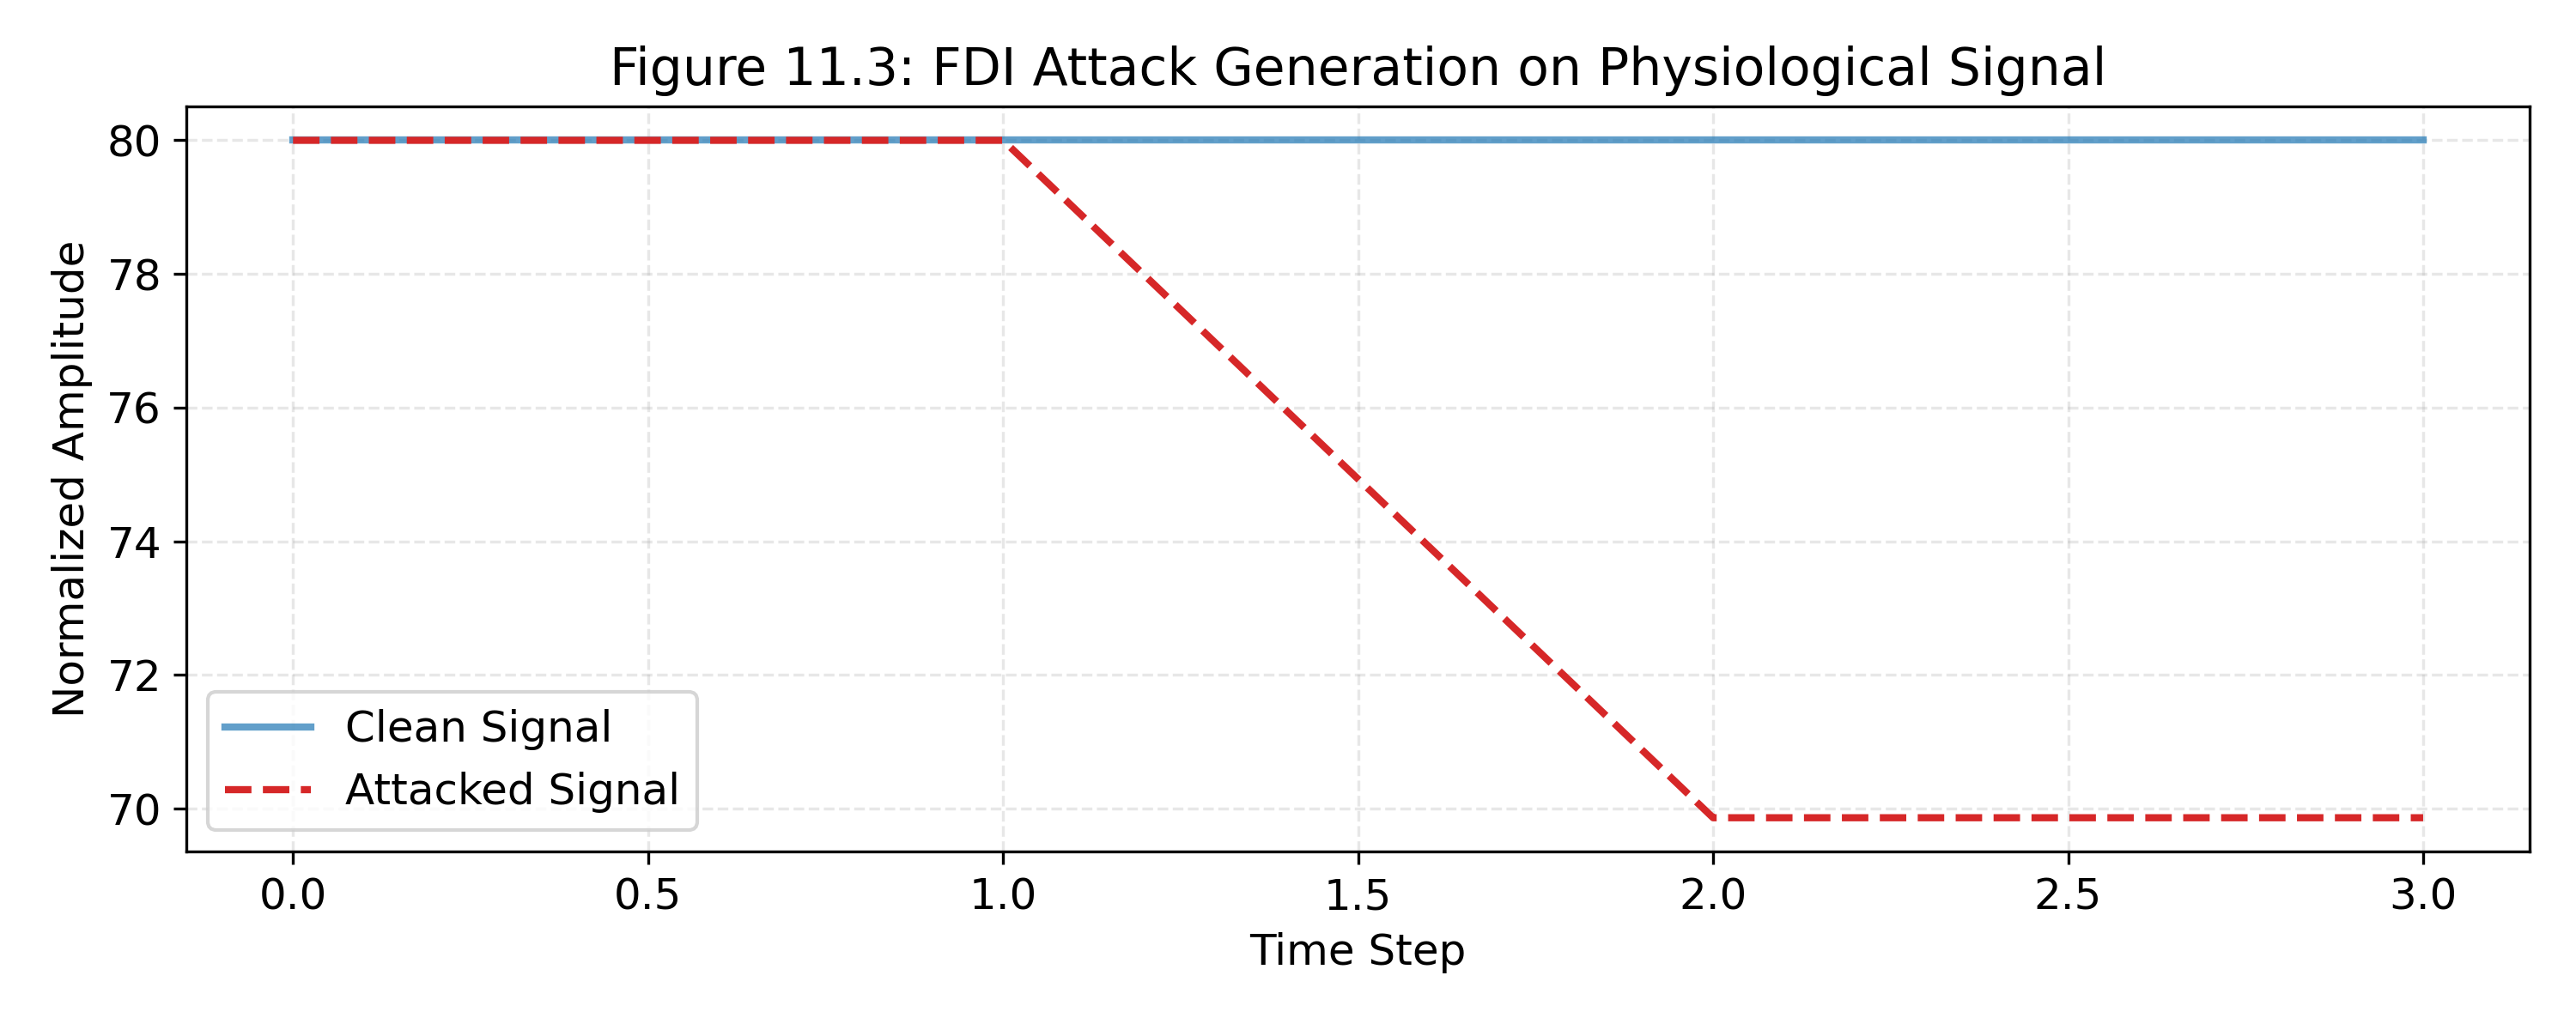
\includegraphics[width=\columnwidth]{figs/Figure_11_3_Attack_Generation.png}
\caption{Illustrative coordinated multi-channel injection: clean signal, attacked signal, and the resulting binary attack mask.}
\end{figure}
Windows are labelled by attack composition: clean (no injection), single-channel, coordinated two-channel, and coordinated three-channel. In coordinated cases the direction and severity of the perturbations are coupled to mimic physiological synchrony. A window is labelled positive if the injection mask is non-empty at any coordinate: y = 1 if attack\_mask.any() else 0.
\section{Data and Preprocessing}
Two datasets were used, chosen to span clinical and wearable monitoring.
\begin{itemize}
\item PhysioNet/CinC Challenge 2012 \cite{silva2012}: irregular, sparse, asynchronous multi-parameter ICU recordings. Four to five core cardiovascular and respiratory parameters with dense sampling were retained, including heart rate (HR), invasive and non-invasive blood pressure (NISysABP, NIDiasABP, NIMAP) and temperature.
\item WESAD \cite{schmidt2018}: high-frequency, synchronised wearable recordings from the RespiBAN chest device. The original stress/amusement labels were discarded; the clean physiology is used purely as a substrate on which FDI attacks are injected.
\end{itemize}
Preprocessing is deliberately fixed and shared by every model. Channels within a record are temporally aligned to a common time axis, then resampled: high-frequency wearable signals are down-sampled and asynchronous clinical observations are binned into uniform steps. Missing clinical values are forward-filled for short gaps, and binary observation masks record where the signal was absent. Normalisation uses per-channel z-scores whose mean and standard deviation are computed on the training split only and then frozen and applied to validation and test data. Crucially, normalisation is applied before synthetic attack injection, so the standardisation reflects a realistic sensor distribution rather than the attack.
Aligned series are segmented into fixed-length rolling windows of T = 120 steps (30 s for WESAD), giving an input tensor X $\in$ $\mathbb{R}$^(B$\times$T$\times$C) where B is batch size. The window length is a compromise: long enough to contain both fast dynamics (heart-rate variability) and slower cycles (respiration), short enough to localise an alert.
\section{Method}
All three models share one temporal encoder and differ only in how channel representations are combined. Freezing the encoder is what makes the comparison an ablation of the fusion mechanism rather than of representation capacity.
\subsection{Shared Temporal Encoder}
Each channel i is encoded independently by a one-dimensional convolutional network followed by a bidirectional gated recurrent unit \cite{cho2014}. Batch normalisation is applied between layers \cite{ioffe2015}. The encoder maps the raw window for that channel to a dense representation z\_i $\in$ $\mathbb{R}$^256 that summarises its temporal morphology.
\subsection{Model A: Naive Multi-Channel Fusion}
Model A is the standard multi-variate classifier. The per-channel embeddings are flattened into a single vector z\_flat = [z\_1, $\ldots$, z\_C] and passed through a multi-layer perceptron. Model A sees all channels at once but receives no structural prior about which channels are physiologically related; any relational structure must be discovered implicitly.
\subsection{Model B: Graph-Only Message Passing}
Model B replaces flat fusion with message passing \cite{gilmer2017} over a fixed channel graph. For every edge (i, j) in the graph the relation input is the concatenation of the two node embeddings:
\begin{equation}
r_{ij} = [z_i ,\, z_j]
\end{equation}
and a relation MLP (512 $\rightarrow$ 128 $\rightarrow$ 64) produces a message m\_ij. Messages arriving at a node are combined by a permutation-invariant sum, and the pooled graph representation feeds a linear sigmoid classifier.
\subsection{Model C: Cross-Sensor Consistency Modelling (CSCM)}
Model C is the hypothesis under test. It augments the relation input with explicit, hand-engineered consistency arithmetic --- the absolute pairwise difference and the element-wise product:
\begin{equation}
r_{ij} = \big[\, z_i ,\, z_j ,\, |z_i - z_j| ,\, z_i \odot z_j \,\big]
\end{equation}
The expanded representation is passed through a wider relation MLP (1024 $\rightarrow$ 128 $\rightarrow$ 64). The motivation is that |z\_i $-$ z\_j| hands the network a direct ``distance'' between two sensors and z\_i $\odot$ z\_j a multiplicative co-activation, so that decoupled signals during a coordinated attack are easier to expose. Model B is the strict ablation: it must infer any distance or covariance from the raw concatenation on its own.
\subsection{The Physiology-Informed Channel Graph}
Models B and C share a pre-defined adjacency matrix derived from known biological coupling. Edges are added where physiology predicts covariance; for example cardiopulmonary coupling is encoded as a bidirectional edge between heart rate and respiration so that the network is instructed to evaluate the consistency of that specific pair.
\subsection{Training and Threshold Calibration}
All models are trained with binary cross-entropy, with the loss weighted by the ratio of clean to attacked windows in the training set to counter class imbalance. Optimisation uses Adam \cite{kingma2015} and early stopping on validation AUROC. Predicted probabilities are converted to discrete labels with a threshold chosen on the validation split by maximising validation F1; that threshold is then frozen and applied to the test split. Thresholds calibrated on validation data are the reason the reported F1 values are not inflated by test-set tuning.
\subsection{Ablation Design and a Known Confound}
The progression A $\rightarrow$ B $\rightarrow$ C isolates two mechanisms: $\Delta$(B$-$A) measures the value of graph message passing over flat fusion, and $\Delta$(C$-$B) measures the incremental value of the explicit consistency features. To keep the feature ablation clean, the temporal embeddings and network depths were held constant, which means the models were not parameter-matched: Model B has approximately 381K parameters and Model C approximately 448K, roughly 17\% more, because its relation MLP consumes a 1024-dimensional input instead of 512. This capacity difference is an acknowledged confound and is revisited in the threats to validity.
\begin{figure}[t]
\centering
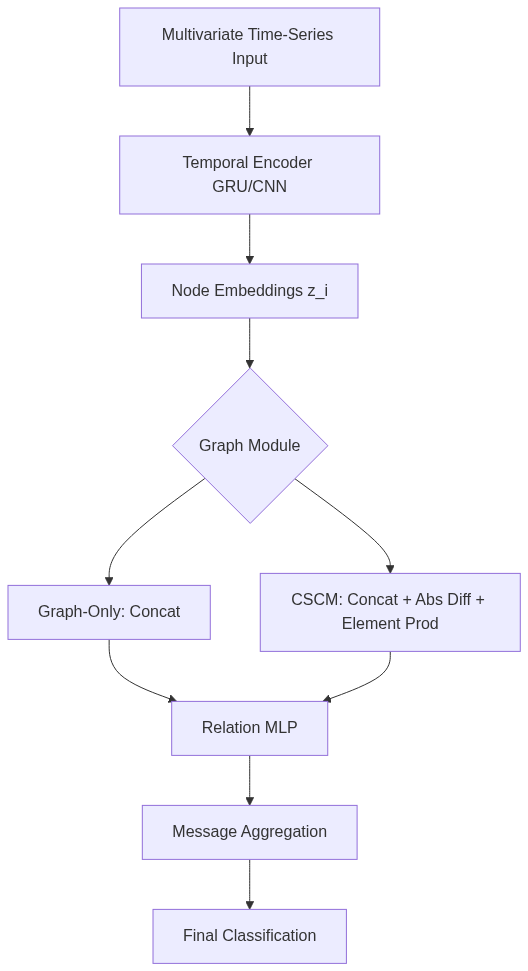
\includegraphics[width=\columnwidth]{figs/Figure_11_5_Architecture.png}
\caption{Model progression: shared temporal encoder feeding (A) flat fusion, (B) graph-only message passing, and (C) CSCM with explicit consistency features.}
\end{figure}
\section{Experimental Setup}
Leakage control. Data were split at the subject or record level, never at the window level, so that no patient appears in both training and test data. For PhysioNet the split key is the RecordID; for WESAD it is the SubjectID. Subjects were shuffled with a fixed seed and partitioned 70\% train, 15\% validation, 15\% test. All attack generation and evaluation used these frozen splits.
Normalisation and thresholds. Per-channel normalisation statistics were computed on the training split only. The decision threshold was tuned on the validation split only. Both are forms of leakage that are easy to introduce accidentally and are explicitly avoided here.
Metrics. With heavy class imbalance, accuracy is uninformative, so we report window-level F1, area under the precision-recall curve (AUPRC) and area under the ROC curve (AUROC). AUPRC is the most sensitive to the minority class; AUROC is included for comparability with prior work. Metrics were computed with scikit-learn \cite{pedregosa2011}.
Seeds and statistics. Every model was trained with three random seeds (42, 123, 2024) to separate architecture effects from initialisation luck. Differences were assessed with a hierarchical paired bootstrap of 1,000 resamples drawn at the subject level, which preserves the intra-patient correlation that window-level resampling would destroy, and with McNemar's test with continuity correction on the paired thresholded predictions. A 95\% confidence interval for $\Delta$ that excludes zero is treated as evidence of a reliable difference.
\begin{table}[t]
\caption{Evaluation substrate. Test windows are pooled across the three seeds.}
\label{tab:8}
\centering
\small
\begin{tabular}{lccccc}
\toprule
Dataset & Setting & Sensors & Split unit & Seeds & Test windows (pooled) \\
\midrule
PhysioNet/CinC 2012 & ICU clinical & Asynchronous clinical observations & RecordID & 3 & 6,501 \\
WESAD & Wearable laboratory & RespiBAN chest sensor & SubjectID & 3 & 1,719 \\
\bottomrule
\end{tabular}
\end{table}
\section{Results}
\subsection{Absolute Performance}
Table II reports accuracy averaged over the three seeds. On the clinical PhysioNet corpus, Model B (graph-only) is the strongest model on all three metrics; Model C does not recover the gap. On the wearable WESAD corpus, Model B has the best AUPRC and AUROC while Model C has a marginally higher F1, and all margins are within one standard deviation. The AUROC values on WESAD cluster near 0.68, which means the models are close to chance at ranking attacked windows above clean ones.
\begin{table}[t]
\caption{Absolute performance (mean $\pm$ std over three seeds). Best value per dataset-metric in bold.}
\label{tab:8}
\centering
\small
\begin{tabular}{lcccc}
\toprule
Dataset & Model & F1 & AUPRC & AUROC \\
\midrule
PhysioNet & A (Naive) & 0.8788 $\pm$ 0.0019 & 0.9550 $\pm$ 0.0008 & 0.8946 $\pm$ 0.0017 \\
PhysioNet & B (Graph-Only) & 0.8863 $\pm$ 0.0031 & 0.9583 $\pm$ 0.0012 & 0.9029 $\pm$ 0.0021 \\
PhysioNet & C (CSCM) & 0.8827 $\pm$ 0.0030 & 0.9556 $\pm$ 0.0019 & 0.8962 $\pm$ 0.0036 \\
WESAD & A (Naive) & 0.8509 $\pm$ 0.0033 & 0.8820 $\pm$ 0.0087 & 0.6812 $\pm$ 0.0183 \\
WESAD & B (Graph-Only) & 0.8489 $\pm$ 0.0068 & 0.8877 $\pm$ 0.0035 & 0.6909 $\pm$ 0.0110 \\
WESAD & C (CSCM) & 0.8520 $\pm$ 0.0008 & 0.8822 $\pm$ 0.0015 & 0.6806 $\pm$ 0.0051 \\
\bottomrule
\end{tabular}
\end{table}
\subsection{Architectural Ablation}
Table III isolates the two mechanisms. Moving from naive fusion to graph message passing ($\Delta$(B$-$A)) is positive on PhysioNet across all three metrics and mixed on WESAD, where the F1 change is slightly negative but AUROC and AUPRC improve. Moving from graph-only to the full CSCM model ($\Delta$(C$-$B)) is consistently negative on PhysioNet and mixed on WESAD. In other words, the explicit consistency arithmetic does not add value on top of graph structure, and on the clinical dataset it costs accuracy.
\begin{table}[t]
\caption{Architectural differences (mean $\Delta$ across seeds).}
\label{tab:8}
\centering
\small
\begin{tabular}{lcccc}
\toprule
Dataset & Comparison & $\Delta$ F1 & $\Delta$ AUPRC & $\Delta$ AUROC \\
\midrule
PhysioNet & $\Delta$(B$-$A) Graph vs Naive & +0.0075 & +0.0033 & +0.0082 \\
PhysioNet & $\Delta$(C$-$B) CSCM vs Graph & $-$0.0035 & $-$0.0027 & $-$0.0067 \\
WESAD & $\Delta$(B$-$A) Graph vs Naive & $-$0.0020 & +0.0058 & +0.0097 \\
WESAD & $\Delta$(C$-$B) CSCM vs Graph & +0.0030 & $-$0.0055 & $-$0.0103 \\
\bottomrule
\end{tabular}
\end{table}
\subsection{Seed-Level Variation}
Averaging hides seed noise, so Table IV reports F1 for every seed. Graph-only is the best model at seed 42 on PhysioNet and at seeds 42 and 2024 on WESAD, ties at the ceiling on the two WESAD seeds where all models reach 0.8529, and is beaten by CSCM at PhysioNet seed 123. The WESAD ties are informative: several models converge on the same discrete F1 because the validation-selected threshold labels almost everything positive, which is consistent with the near-chance AUROC.
\begin{figure}[t]
\centering
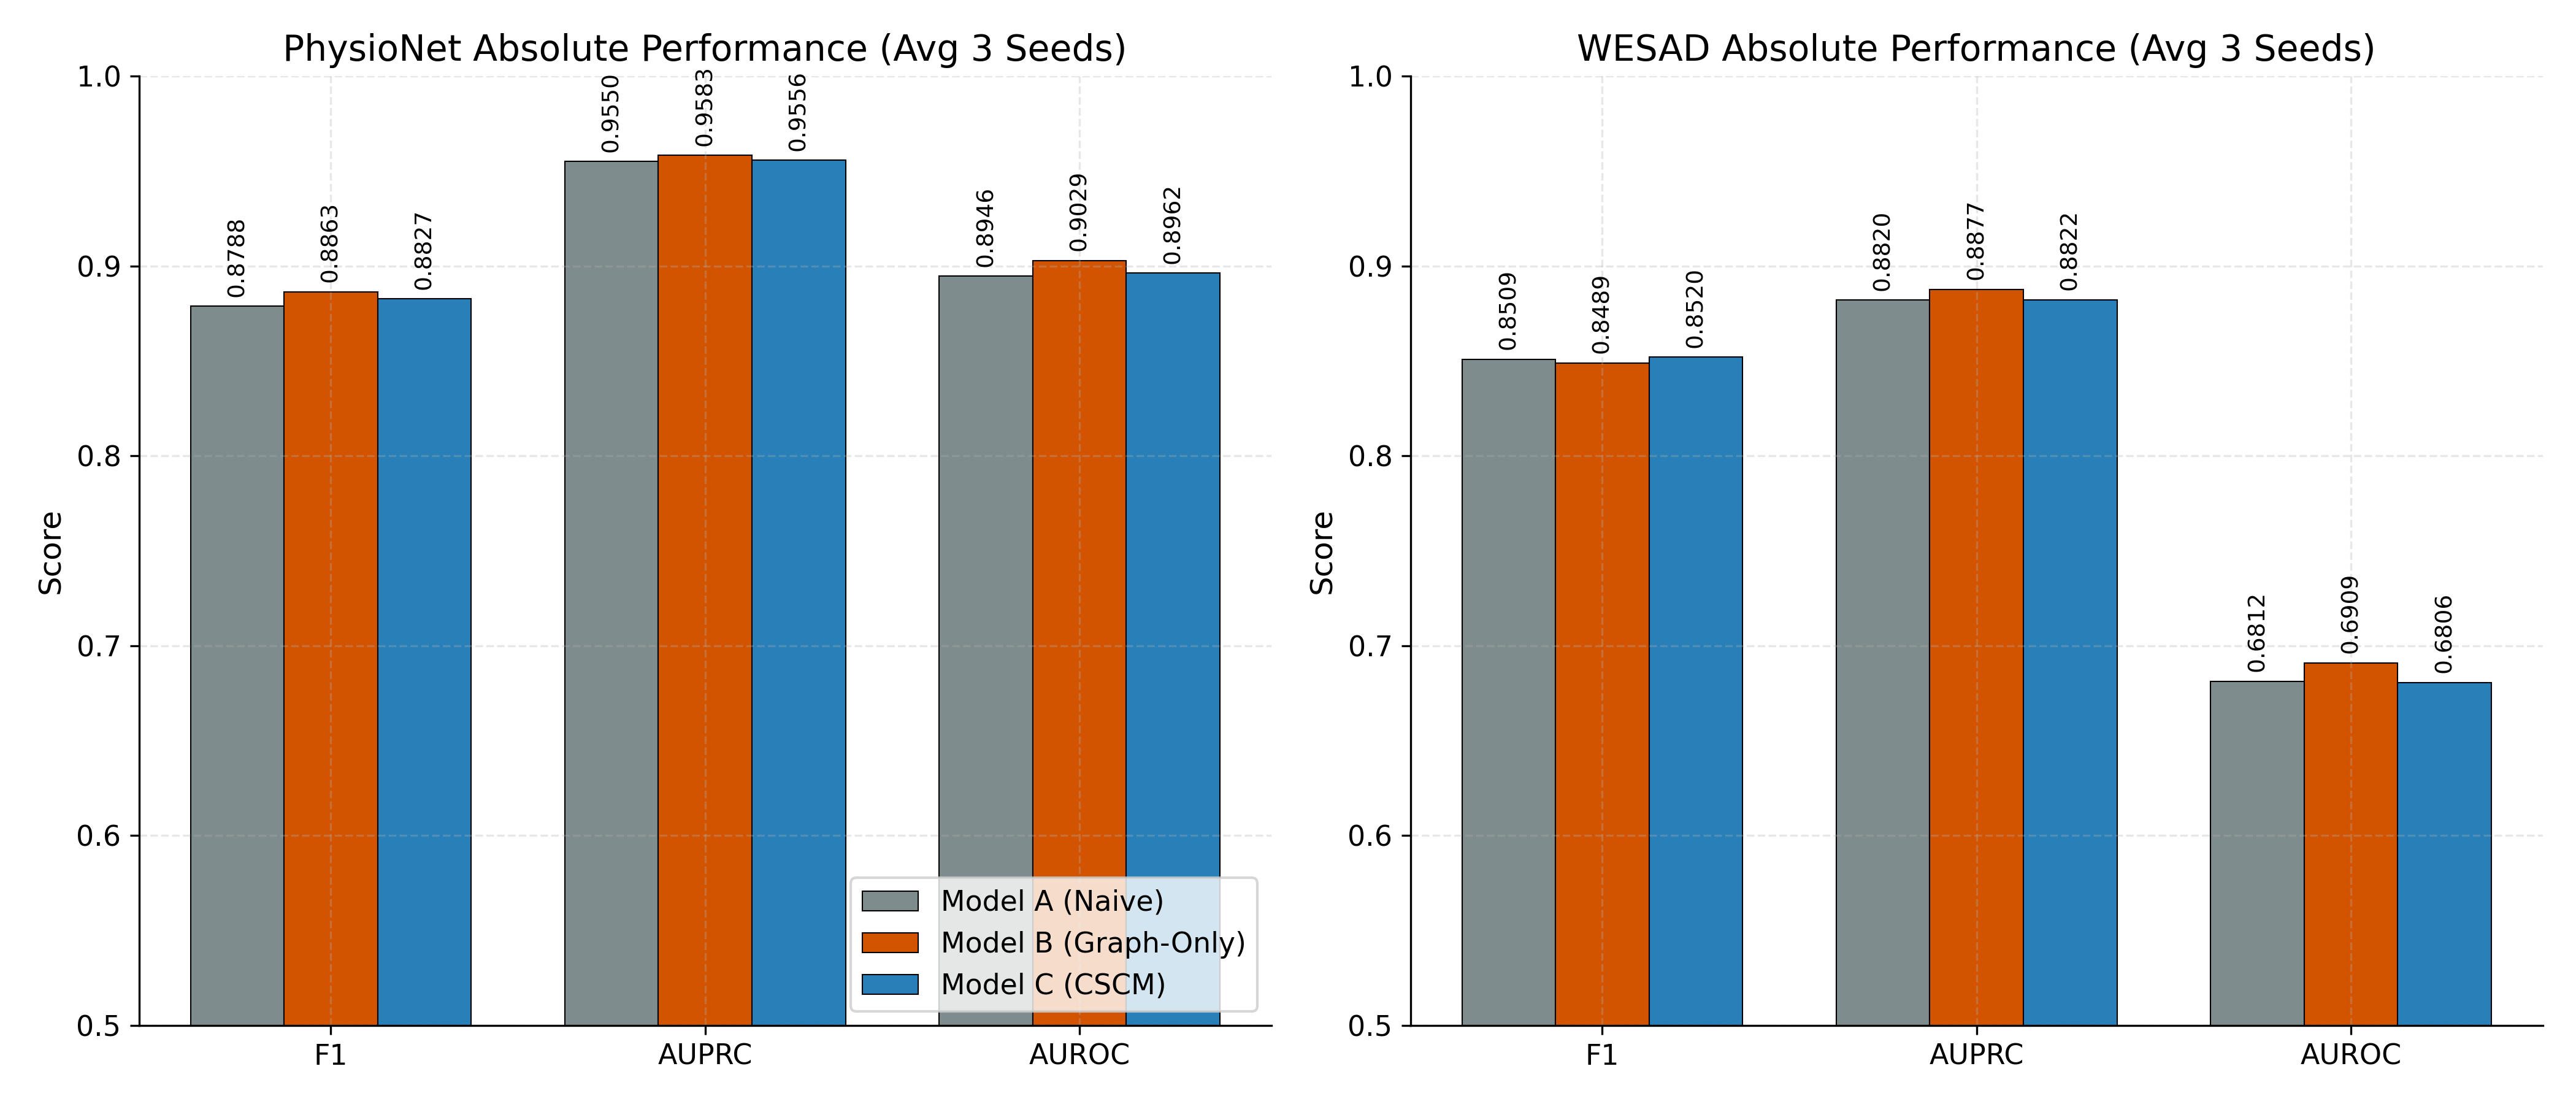
\includegraphics[width=\columnwidth]{figs/absolute_performance_bars.png}
\caption{Absolute F1, AUPRC and AUROC for models A, B and C on both datasets (mean over three seeds).}
\end{figure}
\begin{table}[t]
\caption{F1 score for each model and seed.}
\label{tab:8}
\centering
\small
\begin{tabular}{lcccc}
\toprule
Dataset & Seed & A (Naive) & B (Graph-Only) & C (CSCM) \\
\midrule
PhysioNet & 42 & 0.8807 & 0.8888 & 0.8793 \\
PhysioNet & 123 & 0.8787 & 0.8828 & 0.8851 \\
PhysioNet & 2024 & 0.8770 & 0.8872 & 0.8838 \\
WESAD & 42 & 0.8529 & 0.8529 & 0.8514 \\
WESAD & 123 & 0.8471 & 0.8411 & 0.8517 \\
WESAD & 2024 & 0.8529 & 0.8529 & 0.8529 \\
\bottomrule
\end{tabular}
\end{table}
\subsection{Statistical Reliability}
Table V reports the paired bootstrap intervals and McNemar results. Only two comparisons are reliable. On PhysioNet at seed 2024 the graph model beats naive fusion with a 95\% interval for $\Delta$F1 of [0.0018, 0.0187] and a McNemar p of 0.0003, so graph structure does help on that initialisation. On PhysioNet at seed 42, CSCM is reliably worse than graph-only, with an interval of [$-$0.0180, $-$0.0005] and p = 0.0198. Every other comparison has an interval spanning zero, and the WESAD McNemar tests are degenerate because both models make almost identical discrete predictions. The honest reading is that graph message passing yields a small, seed-dependent gain on clinical data, and that explicit consistency features yield nothing reliable anywhere.
\begin{figure}[t]
\centering
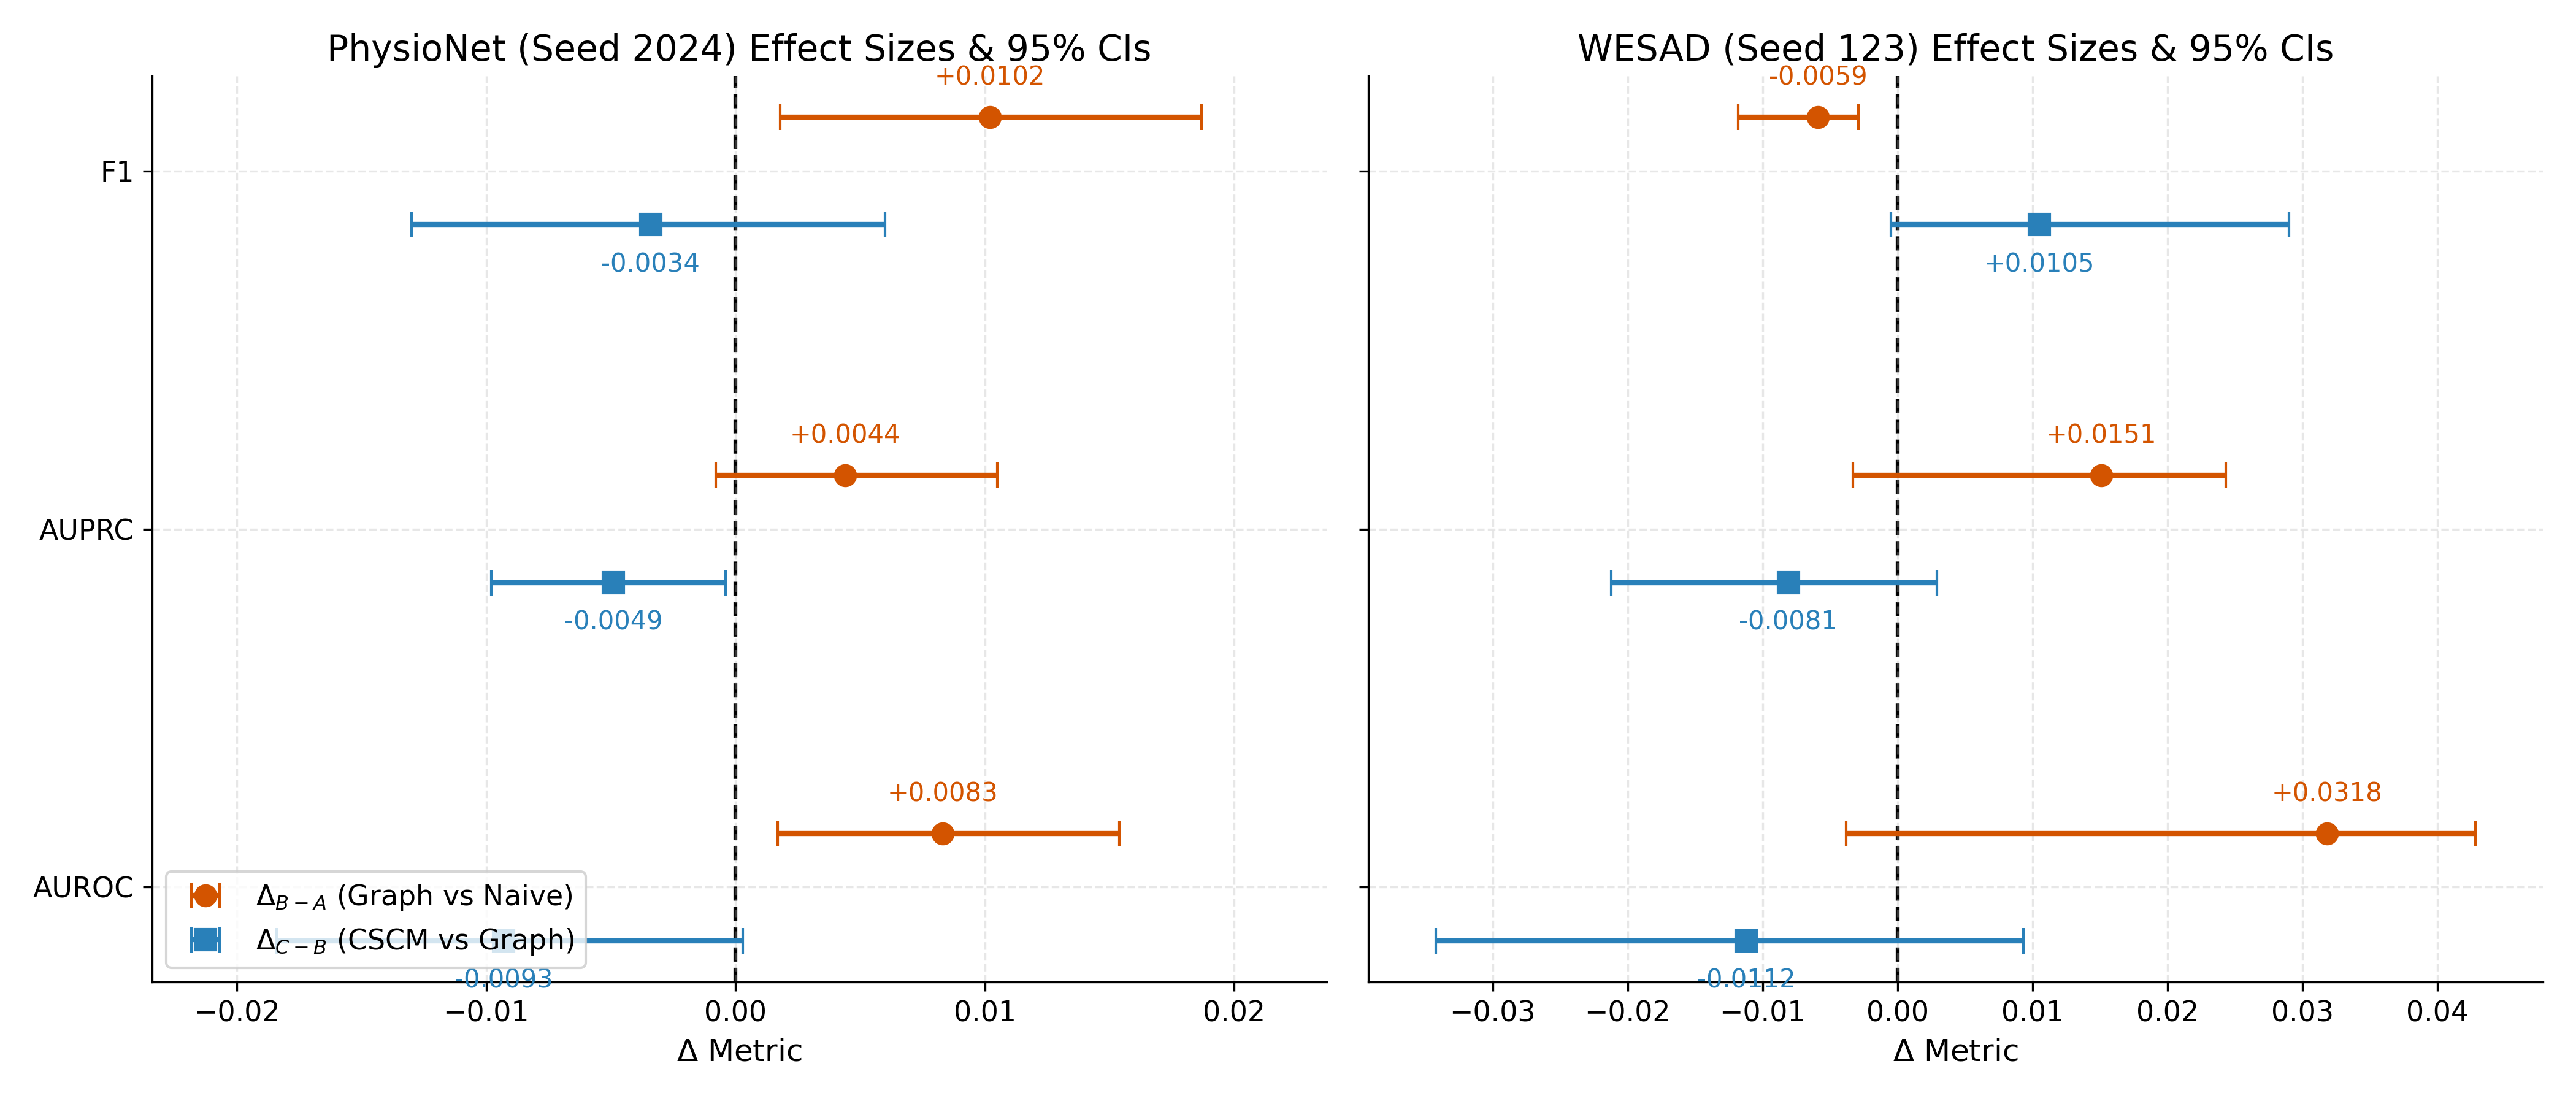
\includegraphics[width=\columnwidth]{figs/effect_size_cis.png}
\caption{Effect sizes for graph-vs-naive and CSCM-vs-graph with 95\% bootstrap confidence intervals.}
\end{figure}
\begin{table}[t]
\caption{Paired bootstrap 95\% CIs for $\Delta$F1 and McNemar test on thresholded predictions.}
\label{tab:8}
\centering
\small
\begin{tabular}{lcccc}
\toprule
Dataset / Seed & Comparison & $\Delta$F1 95\% CI & McNemar p & Reading \\
\midrule
PhysioNet / 42 & C $-$ B & [$-$0.0180, $-$0.0005] & 0.0198 & CSCM reliably worse \\
PhysioNet / 123 & B $-$ A & [$-$0.0038, 0.0118] & 0.360 & Not significant \\
PhysioNet / 123 & C $-$ B & [$-$0.0078, 0.0116] & 0.508 & Not significant \\
PhysioNet / 2024 & B $-$ A & [0.0018, 0.0187] & 0.0003 & Graph reliably better \\
PhysioNet / 2024 & C $-$ B & [$-$0.0130, 0.0060] & 0.443 & Not significant \\
WESAD / all seeds & B $-$ A, C $-$ B & all span zero & $\geq$ 0.49 & Not significant \\
\bottomrule
\end{tabular}
\end{table}
\subsection{Error and Failure Analysis}
Because graph-only is the best model, the failure analysis focuses on it, pooling predictions across seeds. Table VI breaks PhysioNet performance down by attack family and by missingness. Detection is best on drift (F1 0.9289) and additive attacks (0.9220) and weakest on multiplicative attacks (0.9046). Coordinated attacks are harder than single-channel attacks, which confirms that coupling the perturbations across sensors achieves the adversary's goal. Windows containing missing values are detected less well (F1 0.8615) than fully observed windows (0.8927), because forward-filling preserves shape but not information.
\begin{table}[t]
\caption{PhysioNet error analysis for the graph-only model, pooled over seeds.}
\label{tab:8}
\centering
\small
\begin{tabular}{lccc}
\toprule
Subgroup & Recall & Precision & F1 \\
\midrule
Single-channel attack & 0.9068 & 0.9293 & 0.9179 \\
Coordinated 2-channel & 0.8974 & 0.8656 & 0.8812 \\
Coordinated 3-channel & 0.9046 & 0.8259 & 0.8635 \\
Additive & 0.9103 & 0.9340 & 0.9220 \\
Multiplicative & 0.8792 & 0.9316 & 0.9046 \\
Drift & 0.9358 & 0.9221 & 0.9289 \\
Fully observed windows & 0.9120 & 0.8743 & 0.8927 \\
Windows containing NaNs & 0.8956 & 0.8299 & 0.8615 \\
\bottomrule
\end{tabular}
\end{table}
Table VII isolates channel discriminability using single-channel attacks only. Performance is reasonable and fairly even across the PhysioNet channels, whereas the wearable data expose a stark edge case: attacks localised to the respiration channel are never detected, with recall 0.0000. This is a sparse-positive failure. When the attacked channel is inherently sparse and morphologically unlike the dense cardiovascular signals, the relation network appears to discount its embedding entirely rather than flag the inconsistency.
\begin{table}[t]
\caption{Channel breakdown on single-channel attacks (graph-only model, pooled over seeds).}
\label{tab:8}
\centering
\small
\begin{tabular}{lccc}
\toprule
Channel & Recall & Precision & F1 \\
\midrule
HR (PhysioNet) & 0.9061 & 0.9655 & 0.9349 \\
NIMAP (PhysioNet) & 0.9326 & 0.9121 & 0.9222 \\
NISysABP (PhysioNet) & 0.8977 & 0.9368 & 0.9168 \\
NIDiasABP (PhysioNet) & 0.8902 & 0.9289 & 0.9091 \\
Temp (PhysioNet) & 0.9074 & 0.8950 & 0.9011 \\
chest\_Resp (WESAD) & 0.0000 & 0.0000 & 0.0000 \\
\bottomrule
\end{tabular}
\end{table}
Finally, Table VIII compares the discrete decisions of the two graph models. They agree on 89.31\% of PhysioNet windows. Among disagreements, graph-only is correct more often than CSCM, which mirrors the statistical ablation: the extra consistency arithmetic does not systematically buy correct decisions, and it loses slightly more often than it wins.
\begin{table}[t]
\caption{Disagreement between graph-only (B) and CSCM (C) on PhysioNet, pooled over seeds.}
\label{tab:8}
\centering
\small
\begin{tabular}{lcc}
\toprule
Outcome & Windows & Share \\
\midrule
Both correct & 5,039 & 77.51\% \\
Both wrong & 767 & 11.80\% \\
B correct, C wrong & 377 & 5.80\% \\
C correct, B wrong & 318 & 4.89\% \\
\bottomrule
\end{tabular}
\end{table}
\section{Discussion}
Graph structure is the useful inductive bias. The clearest positive result is that forcing the model to evaluate biologically justified channel pairs, rather than discovering relations implicitly from a flat vector, improves detection on the clinical dataset. The gain is small --- on the order of one F1 point --- but it is statistically visible at one seed, and it is consistent in sign across the metrics. For noisy, irregular ICU recordings, a structural prior appears to help the network extract signal.
Explicit consistency arithmetic is redundant. The hypothesis that |z\_i $-$ z\_j| and z\_i $\odot$ z\_j would accelerate the relation network is not supported. A plausible explanation is that the relation MLP in the graph-only model, operating on the raw concatenation [z\_i, z\_j], is already expressive enough to approximate whatever non-linear distance boundary matters; supplying the arithmetic explicitly is at best redundant and at worst injects correlated inputs that perturb optimisation. Because Model C also carries about 17\% more parameters, part of its deficit may reflect capacity and optimisation dynamics rather than the features themselves.
The datasets behave differently, and the difference is instructive. On WESAD the signals are clean, high-frequency and already tightly synchronised, and the naive model performs adequately; there is little structure left for a graph to add, and AUROC near chance suggests the windowed task itself is hard on this substrate. On PhysioNet the signals are sparse and noisy, and modelling relations pays off. This suggests that cross-sensor modelling is most valuable exactly where clinical monitoring is least forgiving.
The failure modes are as important as the averages. Attacks on sparse channels can be missed entirely, missing physiological data degrades detection, and coordinated attacks remain harder than single-channel ones even for a model that is explicitly given the channel graph. A system that reported only the mean F1 would hide all three.
\section{Threats to Validity}
Construct validity. Attacks are synthetic. They are drawn from additive, multiplicative and drift families and are clipped to remain physiologically plausible, which is the right control for testing evasion of threshold monitors, but they are not real attacks. A generative adversary producing organic coordinated signals has not been tested.
Internal validity. The B-versus-C ablation is confounded by parameters, since Model C is about 17\% larger. The conclusion that explicit consistency features are unnecessary is therefore conditional on the parameterisations tested. Only three seeds were used, and one seed is not enough to declare a winner.
External validity. Two datasets, both public, both with a single frozen split and a single injection configuration, bound how far the results generalise. Cross-dataset transfer was not tested.
Reporting. All figures quoted here are taken from the project's own metric CSVs and the pooled error analysis, not re-derived from scratch. The pipeline is deterministic given the seeds, so the numbers are reproducible, but they have not been reproduced by an independent party.
\section{Conclusion and Future Work}
We asked whether physiology-aware cross-sensor consistency modelling improves detection of coordinated multi-channel FDI attacks over naive multi-channel fusion, and tested it under a leakage-controlled protocol on clinical and wearable data. The answer is a qualified no. Graph message passing over a physiology-informed channel graph is a real, if modest, advantage on clinical recordings; hand-engineered consistency arithmetic adds nothing reliable and can hurt. On clean wearable data none of the three architectures separates from the others.
We report this as a benchmark rather than a defeat. The protocol is fully specified, the effect sizes and their uncertainty are reported, and the failure cases are named. Future work should add published FDI detectors as external baselines, run more seeds with a pre-registered power analysis, replace the forward-fill missing-data strategy with a missingness-aware encoder, use a generative attack model, and test cross-dataset transfer. If explicit consistency features help anywhere, these are the conditions most likely to reveal it.
\bibliographystyle{IEEEtran}
\begin{thebibliography}{99}
\bibitem{liu2011}
M. K. Liu, P. Ning, and M. K. Reiter, ``False data injection attacks against state estimation in electric power grids,'' ACM Trans. Inf. Syst. Secur., vol. 14, no. 1, pp. 1--33, 2011.
\bibitem{mo2012}
Y. Mo, T. H.-J. Kim, K. Brancik, D. Dickinson, H. Lee, A. Perrig, and B. Sinopoli, ``Cyber-physical security of a smart grid infrastructure,'' Proc. IEEE, vol. 100, no. 1, pp. 195--209, 2012.
\bibitem{alsubaei2017}
F. Alsubaei, A. Abuhussein, and S. Shiva, ``Security and privacy in the Internet of Medical Things: Taxonomy and risk assessment,'' in Proc. IEEE 42nd Conf. Local Comput. Netw. Workshops (LCN Workshops), 2017, pp. 112--120.
\bibitem{chalapathy2019}
R. Chalapathy and S. Chawla, ``Deep learning for anomaly detection: A survey,'' arXiv:1901.03407, 2019.
\bibitem{kipf2017}
T. N. Kipf and M. Welling, ``Semi-supervised classification with graph convolutional networks,'' in Proc. ICLR, 2017.
\bibitem{gilmer2017}
J. Gilmer, S. S. Schoenholz, P. F. Riley, O. Vinyals, and G. E. Dahl, ``Neural message passing for quantum chemistry,'' in Proc. ICML, 2017, pp. 1263--1272.
\bibitem{battaglia2018}
P. W. Battaglia et al., ``Relational inductive biases, deep learning, and graph networks,'' arXiv:1806.01261, 2018.
\bibitem{cho2014}
K. Cho, B. van Merriënboer, C. Gulcehre, D. Bahdanau, F. Bougares, H. Schwenk, and Y. Bengio, ``Learning phrase representations using RNN encoder-decoder for statistical machine translation,'' in Proc. EMNLP, 2014, pp. 1724--1734.
\bibitem{hochreiter1997}
S. Hochreiter and J. Schmidhuber, ``Long short-term memory,'' Neural Comput., vol. 9, no. 8, pp. 1735--1780, 1997.
\bibitem{silva2012}
I. Silva, G. Moody, D. J. Scott, L. A. Celi, and R. G. Mark, ``Predicting in-hospital mortality of ICU patients: The PhysioNet/Computing in Cardiology Challenge 2012,'' in Proc. Comput. Cardiol., 2012, pp. 245--248.
\bibitem{schmidt2018}
P. Schmidt, A. Reiss, R. Duerichen, C. Marberger, and K. Van Laerhoven, ``Introducing WESAD, a multimodal dataset for wearable stress and affect detection,'' in Proc. ACM Int. Conf. Multimodal Interaction (ICMI), 2018, pp. 400--408.
\bibitem{paszke2019}
A. Paszke et al., ``PyTorch: An imperative style, high-performance deep learning library,'' in Proc. NeurIPS, 2019, pp. 8024--8035.
\bibitem{fey2019}
M. Fey and J. E. Lenssen, ``Fast graph representation learning with PyTorch Geometric,'' in Proc. ICLR Workshop, 2019.
\bibitem{kingma2015}
D. P. Kingma and J. Ba, ``Adam: A method for stochastic optimization,'' in Proc. ICLR, 2015.
\bibitem{ioffe2015}
S. Ioffe and C. Szegedy, ``Batch normalization: Accelerating deep network training by reducing internal covariate shift,'' in Proc. ICML, 2015, pp. 448--456.
\bibitem{pedregosa2011}
F. Pedregosa et al., ``Scikit-learn: Machine learning in Python,'' J. Mach. Learn. Res., vol. 12, pp. 2825--2830, 2011.
\bibitem{efron1993}
B. Efron and R. J. Tibshirani, An Introduction to the Bootstrap. New York, NY, USA: Chapman \& Hall/CRC, 1993.
\bibitem{dietterich1998}
T. G. Dietterich, ``Approximate statistical tests for comparing supervised classification learning algorithms,'' Neural Comput., vol. 10, no. 7, pp. 1895--1923, 1998.
\end{thebibliography}
\end{document}
